\subsection{Недетерминированный конечный автомат (НКА).}

Недетерминированность: Для каждого состояния и входного символа может быть несколько возможных переходов.

\textbf{Ключевое отличие от ДКА}: Функция перехода $\delta$ в НКА возвращает множество состояний, а не одно состояние. Это означает, что при чтении одного символа из текущего состояния НКА может перейти в несколько состояний одновременно, либо не перейти ни в какое.

Мы можем считать, что $S$ - множество стартовых позиций.

Пример НКА:
\begin{center}
    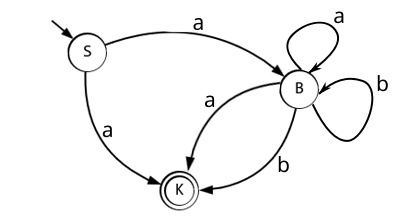
\includegraphics[width = 12cm]{assets/8_1_1.jpg}
\end{center}

Уйдем пока в другую сферу. Как хранить ДКА?

$s$ будем хранить int-ом, $t$ - vector<bool>(n), $\delta$ vector<vector<int> > (n,c). 

И например операцию проверки в нем можно сделать вот так:

\begin{lstlisting}[mathescape]
   bool accept(x){
        cur = s
        for(i=0...len(x)-1)
          cur = delta[cur][x[i]]
        return t[cur]
   }
\end{lstlisting}
Как хранить НКА?

$s$ будем хранить int-ом (или set-ом), $t$ - vector<bool>(n), $\delta$ vector<vector<set<int> >\,> (n,c). 

И например операцию проверки в нем можно сделать вот так:

\begin{lstlisting}[mathescape]
   bool accept(x){
        can[0][s] = true
        for(i = 0... len(x)-1)
            for(q = 0... n-1)
                if can[i][q] \\$\text{можем идти дальше}$
                    for r : delta[q][x[i]]
                        can[i+1][r]=true
        for(q = 0...n-1)
            if(can[len(x)][q] and t[q])
                return true
        return false
   }
\end{lstlisting}

Алгоритм работает за $len(x) n^2$. 

НКА легче строить, но им сложнее оперировать и строиться. То есть в ДКА мы платим сложностью построения, чтобы легко потом проверять на содержание в автомате.

\thmm{Теорема}

Для языка $L$ существует НКА $A_n \Leftrightarrow$ для $L$ существует ДКА $A_D$

\textbf{Доказательство:}

    Очевидно, что ДКА - частный случай НКА, поэтому нам надо доказывать только стрелку в правую сторону.

    \deff{Алгоритм Томпсона.}

    Давайте в том алгоритме, который у нас был сверху сделаем функцию, которая будет брать $i$-ую строчку и будет возвращать $i+1$:
    
    \begin{lstlisting}[mathescape]
     vector<bool> next(vector<bool> a, char c){
        result = vector<bool> (n)
        for(q = 0... n-1)
            if a[q] \\$\text{можем идти дальше}$
                for r : delta[q][c]
                    result[r] = true;
        return result;
   }
    \end{lstlisting}

    И теперь заменим в исходном коде операции НКА на данную функцию:

    \begin{lstlisting}[mathescape]
   bool accept(x){
        can[0][s] = true
        for(i = 0... len(x)-1)
            can[i+1] = next(can[i],x[i])
        for(q = 0...n-1)
            if(can[len(x)][q] and t[q])
                return true
        return false
   }
\end{lstlisting}

    Хмм, что-то похожее на то, что было в ДКА. \sout{У вас копипаста - 5 минусов, делей 3, до свидания}

    Пусть $Q_D = 2^{Q_N}$, $\Sigma$,  $\delta_{D} =(A,c) = \{r \bigm| \exists q \in A, r \in \delta_N(a,c)\}$. $T_D = \{A \bigm| A \cap T_n \neq \varnothing\}$. 
    
    Получили автомат и детерминированный.
    
\hfill Q.E.D.

\subsection{$\varepsilon$ - НКА}


$\varepsilon$-НКА  --- это расширение обычного НКА, позволяющее автомату переходить между состояниями, не потребляя никаких входных символов (так называемые $\varepsilon$ переходы). Это добавляет еще больше гибкости в процесс распознавания языка.

$\varepsilon$ - замыкание:

\begin{enumerate}
    \item  Сделаем транзитивное замыкание по графу $\varepsilon$ - переходов, добавим новые ребра как $\varepsilon$ - переходы.
    
     То есть если $x$ нужно было идти 2 раза подряд по $\varepsilon$ ребру, то теперь всего 1 $\varepsilon$ переход
     \item  Если есть вершины $p,q$, $q$ - терминальная, то сделаем $p$ терминальной. 
     
     Получается, что любое слово, задающееся этим автоматом, такое, что последний переход в терминальное не $\varepsilon$
     \item Рассмотрим вершины $p,q,r$. Пусть из $p$ в $q$ есть $\varepsilon$ переход, а из $q$ в $r$ переход по какому-то символу $c$. Добавим ребро из $p$ в $r$ по $c$. 

     Получается, что любое слово можно допустить без $\varepsilon$-переходов.
     \item удалим $\varepsilon$-переходы и получили обычное НКА.
\end{enumerate}

Мы показали, что любой язык задается через ДКА, НКА, $\varepsilon$-НКА, причем из любого автомата я могу получить любой другой автомат с помощью $\varepsilon$-замыкания или алгоритма Томпсона.


Теперь докажем теорему Клини, ту самую с прошлой лекции. 

\thmm{Теорема (Клини)}

$Reg = Aut$

\textbf{Доказательство:}

\begin{enumerate}
    \item $Reg \subset Aut$

    Хочу доказать, что $\forall i: Reg_i \subset Aut$. Будем считать, что у нас $\varepsilon$-НКА автоматы с одним входом и выходом

    \textbf{База:} $i=0$. Очевидно.

    \textbf{Индукционный переход:}

    Пусть $Reg_i \subset Aut \Rightarrow Reg_{i+1}\subset$.

    Рассмотрим случаи как получился тот или иной язык:
    \begin{enumerate}
        \item $L = A \cup B$: Для $A,B$ мы уже умеем строить автоматы. Давайте сделаем новую стартовую вершину, которая будет вести в стартовые $A,B$, с помощью $\varepsilon$-переходов, а также соединим их терминальные и сделаем еще одну новую вершину терминальной.
        \item $L=AB$: Для $A,B$ мы уже умеем строить автоматы. Соединю $\varepsilon$-переходом конец $A$ и старт $B$. Старт $A$ сделаю стартом нового автомата, а терминальную вершины $B$ соответственно сделаю терминальной вершиной нового автомата.
        \item $L = A^*$. Для $A$ мы уже умеем строить автомат. Добавлю стартовое состояние, которое ведет ($\varepsilon$-переходом) в стартовое состояние $A$. Добавлю новую вершину, в которую я поведу конец $A$ ($\varepsilon$-переходом), и соединю вершины туда обратно.
    \end{enumerate}    
    Все это крайне подробно изображено на рисунке:
    \begin{center}
    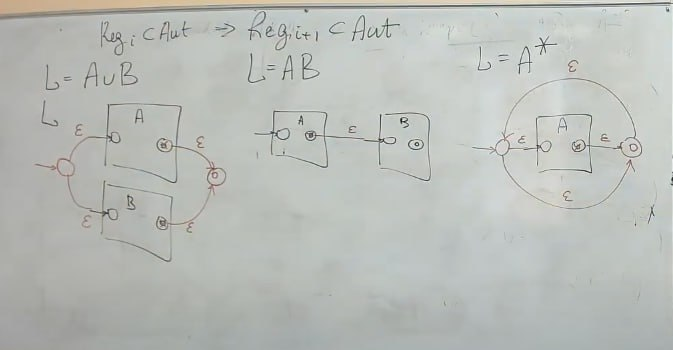
\includegraphics[width = 12cm]{assets/8_2_1.jpg}
\end{center}
    Индукционный переход доказан и первая часть доказательства тоже!

    
\end{enumerate}
